%!TEX root = ../main.tex

\chapter{Euristiche per migliorare l'apprendimento} % (fold)
\label{cha:euristiche_per_migliorare_l'apprendimento}
Per garantire la convergenza di un algoritmo di apprendimento non esistono criteri ben definiti. Ci sono una serie di questioni pratiche e teoriche da affrontare quando si vuole addestrare una rete neurale. Ad esempio: di quanti strati una rete dovrà essere composta, oppure, quante unità devono esserci per ogni strato. Per rispondere a queste domande si introduce il concetto di \textbf{generalizzazione}.

\section{Generalizzazione} % (fold)
\label{sec:generalizzazione}
\begin{mydef}[Generalizzazione]
	Per generalizzazione si intende la capacità di una rete di classificare correttamente esempi mai incontrati all'interno dell'insieme di addestramento (esempi di test).
\end{mydef}
Si assume che gli esempi di test siano tratti dalla stessa popolazione usata per generare il training set. Si introduce dunque un nuovo insieme noto come insieme dei test (\emph{test set}).\\

Il problema di apprendimento può essere visto come un problema di “approssimazione di una curva”. In questo caso la rete è considerata semplicemente come una mappa input/output non lineare, quindi una buona generalizzazione è vista come una buona interpolazione dei dati di input.\\

Una rete progettata per generalizzare bene produce mappature input/output corrette anche se l'input è lievemente differente dagli esempi usati in fase di training; se però la rete viene addestrata con troppi esempi, si rischia di memorizzare il training set; la rete cioè apprende il \emph{rumore} presente nel training set. Questo fenomeno è detto \textbf{overfitting} o \textbf{overtraining}. Una rete “sovra-addestrata” è troppo rigida e pertanto perde la capacità di generalizzazione.\\

\emph{In generale} una rete troppo piccola impara poco, mentre una rete troppo grande impara molto, ma non generalizza abbastanza. In entrambi i casi si rischia di non riuscire a risolvere il problema. È, dunque, necessario trovare un \textbf{giusto compromesso}. 

\newpage

Dal momento che stiamo considerando l'apprendimento come un'approssimazione di una curva, il compromesso precedente può essere visto sotto il seguente profilo: troppi pochi parametri e.g. $y=ax + b$ non permettono di risolvere il problema, mentre con troppi parametri e.g. $y=ax^3 + bx^2 + cx + d$ si rischia l'overfitting.

\begin{figure}[h!]
	\centering
	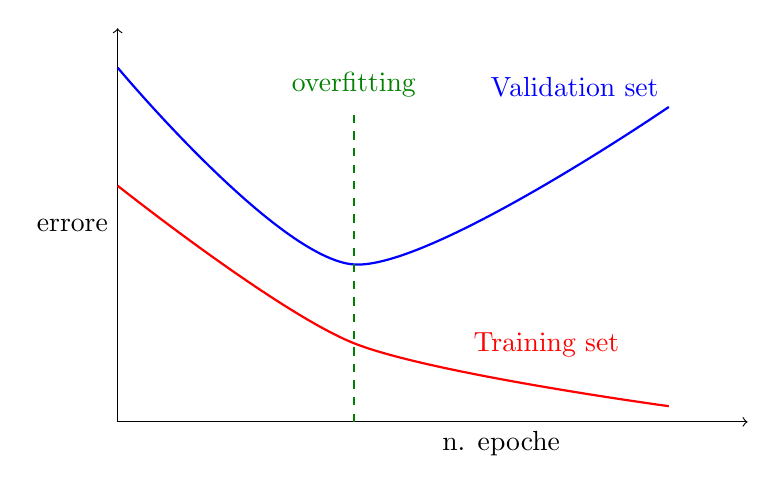
\begin{tikzpicture}
		\draw[->] (0,0) -- node[left] {errore} (0,5);
		\draw[->,below right] (0,0) -- node {n. epoche} (8,0);

		\draw[thick, color=blue] plot [smooth, tension=0.5] coordinates{(0, 4.5) (3, 2) (7, 4)} node[above left] {Validation set};
		\draw[thick, color=red] plot [smooth, tension=0.5] coordinates{(0, 3) (3, 1) (7, 0.2)} node[above left=0.5cm] {Training set};
        
		\draw[thick, color=green!50!black, dashed] (3, 0) -- (3, 4) node[above] {overfitting};
        
	\end{tikzpicture}
	\caption[Andamento dell'errore e overfitting]{La curva blu mostra l'andamento dell'errore nel classificare i dati di training, mentre la curva rossa mostra l'errore nel classificare i dati di test o validazione. Se l'errore di validazione aumenta mentre l'errore sui dati di training diminuisce, ciò indica che siamo in presenza di un possibile caso di overfitting.}
\end{figure}

\begin{figure}[h!]
	\centering
	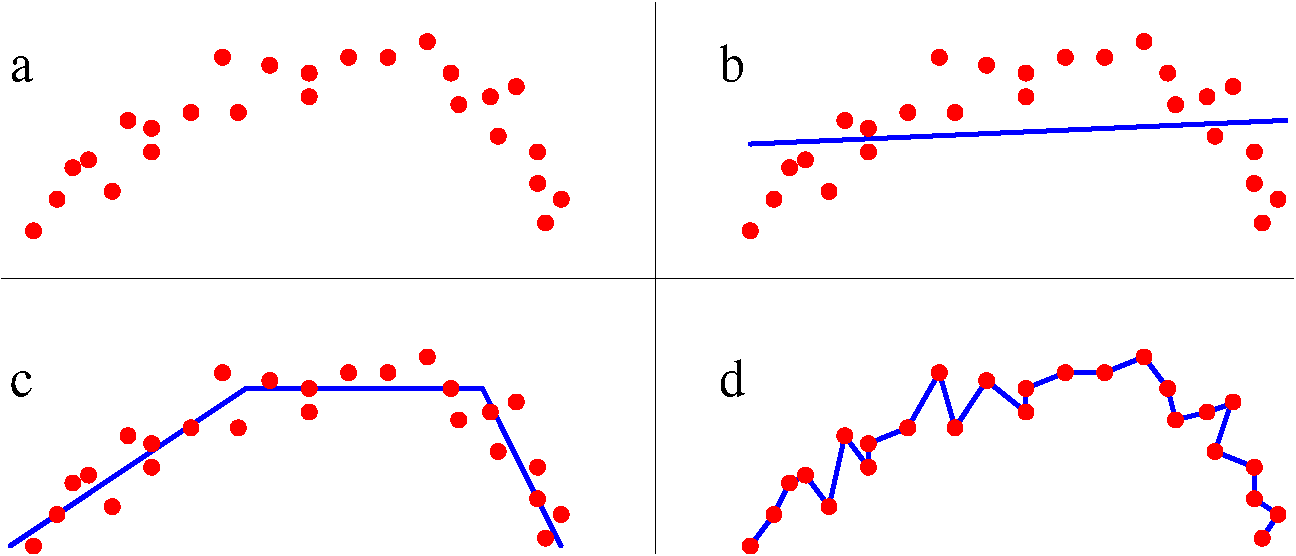
\includegraphics[width=10cm]{images/overfit2}
	\caption[Interpolazione e overfitting]{(a) dati del training set, (b) sotto approssimazione, (c) una buona stima sui dati, (d) overfitting: la curva di apprendimento è perfettamente disposta sul training set.}
\end{figure}

La capacità di generalizzazione è influenzata da tre fattori principali: le dimensioni del training set, l'architettura della rete neurale e la complessità del problema.

\newpage

Alla luce del fatto che non si ha alcun controllo sulla complessità del problema, è possibile affrontare il problema della generalizzazione sotto due punti di vista differenti:
\begin{enumerate}
	\item l'architettura della rete è prefissata e lo scopo è determinare una dimensione del training set ottimale per una buona generalizzazione;
	\item la dimensione del training set è prefissata e lo scopo è di determinare la migliore architettura di rete per una buona generalizzazione.
\end{enumerate}

% section generalizzazione (end)


\section{Cross-validation} % (fold)
\label{sec:cross_validation}
Si introduce ora uno strumento per risolvere il problema della selezione dell’architettura della rete neurale; più precisamente questo strumento consente, dato un insieme di possibili modelli, di scegliere quello migliore secondo certi criteri.
Inizialmente il set di dati viene ripartito in modo random in un training set e un test set. Il training set è ulteriormente diviso in due insiemi disgiunti:
\begin{itemize}
	\item \textbf{Estimation subset:} usato per il training del modello;
	\item \textbf{Validation subset:} usato per validare il modello.
\end{itemize}
La motivazione è validare il modello su un set di dati diverso da quello usato per l'addestramento. In questo modo è possibile usare il training set per stimare le prestazioni dei vari modelli candidati e scegliere quindi il migliore. C'è comunque la possibilità che il modello più performante in realtà sia incappato in un overfitting del validation set. Per evitare questo si ricorre al test set per verificare la capacità di generalizzazione della rete.

\newpage

\begin{figure}[h!]
	\centering
	\begin{tikzpicture}[font=\scriptsize]
		\pie[pos={8,0},rotate=90, radius=1.2, color={black!40, black!20}]{75/ E, 25/ V}
		\pie[pos={12,0}, rotate=0, radius=1.2, color={black!40, black!20}]{75/ E, 25/ V}
		\pie[pos={8,-4}, rotate=270, radius=1.2, color={black!40, black!20}]{75/ E, 25/ V}
		\pie[pos={12,-4}, rotate=180, radius=1.2,  color={black!40, black!20}]{75/ E, 25/ V}
	\end{tikzpicture}
	\caption[Cross-validation]{Esempio di cross-validation: partizionamenti del training set in estimation subset E e validation subset V.}
\end{figure}

\subsection{Variante del cross-validation} % (fold)
\label{sub:variante_del_cross_validation}
Quando la dimensione del set di dati è piccola, si può ricorrere al \emph{multifold cross-validation} dividendo il set di $N$ esempi in $K$ sottoinsiemi, $K>1$. Il modello viene poi addestrato su ogni sottoinsieme ad eccezione di uno; quest'ultimo formerà il validation set. Questa procedura viene ripetuta $K$ volte utilizzando per il validation set a turno uno dei $K$ sottoinsiemi. Le prestazioni del modello vengono misurate facendo la media degli errori quadrati sul validation set per ognuna delle $K$ ripetizioni.\\
Lo svantaggio di questa tecnica è che richiede molta computazione dal momento che il modello deve essere addestrato $K$ volte.
Quando il numero di esempi è ancora più piccolo si può ricorrere ad una forma estrema di questa tecnica detta \textbf{leave-one-out} in cui $K=N$.
% subsection variante_del_cross_validation (end)
% section cross_validation (end)

\newpage

\section{Metodo di training “early-stopping”} % (fold)
\label{sec:metodo_di_training_early_stopping_}
Con l’obiettivo di una buona generalizzazione è molto difficile decidere quando è il momento di bloccare il training. C'è il rischio di overfitting dei dati se non si ferma l'addestramento al punto giusto.\\
È possibile evitare il fenomeno dell'overfitting ricorrendo al metodo precedente; l'estimation set viene usato per addestrare la rete e il validation set serve a testarla dopo ogni epoca. Più precisamente il processo procede nel seguente modo:
\begin{itemize}
	\item dopo un periodo di addestramento sull'estimation set, si calcola l'errore di validazione per ogni esempio del validation set;
	\item quando la fase di validazione è completa, si riprende la fase di addestramento per un altro periodo.
\end{itemize}

Se si osserva la sola curva dell'errore dell’estimation set (vedi Figura~\ref{fig:overfit}), questo si riduce all’aumentare delle epoche, e verrebbe naturale pensare di eseguire il training anche oltre il punto di minimo della curva del validation set. In realtà ciò che la rete apprende dopo quel punto è il rumore contenuto nei dati del training/estimation set. Questa euristica suggerisce quindi di fermare l'addestramento in corrispondenza del minimo della curva relativa al validation set.
\begin{figure}[h!]
	\centering
	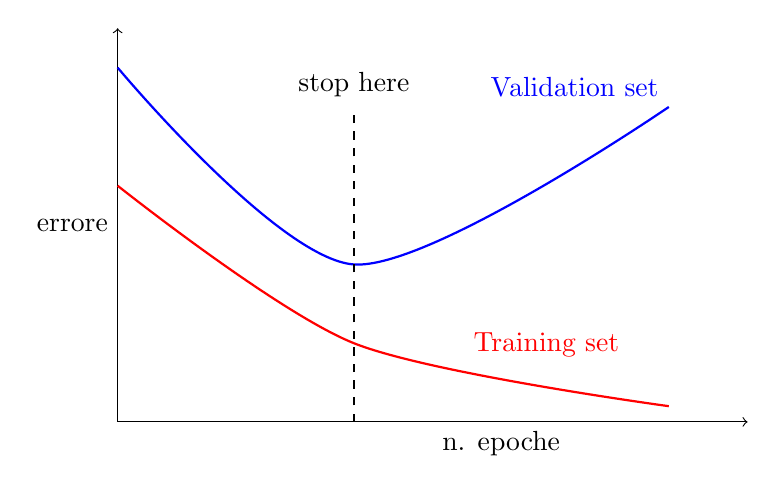
\begin{tikzpicture}
		\draw[->] (0,0) -- node[left] {errore} (0,5);
		\draw[->,below right] (0,0) -- node {n. epoche} (8,0);

		\draw[thick, color=blue] plot [smooth, tension=0.5] coordinates{(0, 4.5) (3, 2) (7, 4)} node[above left] {Validation set};
		\draw[thick, color=red] plot [smooth, tension=0.5] coordinates{(0, 3) (3, 1) (7, 0.2)} node[above left=0.5cm] {Training set};
        
		\draw[thick, dashed] (3, 0) -- (3, 4) node[above] {stop here};
        
	\end{tikzpicture}
	\caption{Andamento di errore e metodo di early stopping.}\label{fig:overfit}
\end{figure}



% section metodo_di_training_early_stopping_ (end)

\newpage

\section{Tecniche di pruning} % (fold)
\label{sec:tecniche_di_pruning}
Le capacità funzionali e di generalizzazione di una determinata rete sono fortemente influenzate dalla sua dimensione (ovvero il numero di neuroni nascosti). Con una rete troppo piccola si rischia di non riuscire a risolvere il problema, mentre con una troppo grande si rischia di apprendere il rumore deteriorando la capacità di generalizzare. È necessario quindi un \textbf{compromesso}.\\

Le tecniche di network pruning hanno lo scopo di minimizzare le dimensioni della rete mantenendo buone prestazioni. È possibile raggiungere questo obiettivo in due modi:
\begin{enumerate}
	\item \textbf{pruning}: si parte da una rete sufficientemente grande per poi ridurla eliminando connessioni sinaptiche o neuroni interi.
	\item \textbf{growing}: si parte da una rete piccola per poi espanderla;
\end{enumerate}
La prima tecnica di solito è più veloce in termini di numero di epoche (convergenza più veloce), ma richiede maggior peso computazionale dal momento che ci sono più unità. Ad ogni modo questo metodo è il più adottato.

\begin{figure}[h!]
	\centering
	\begin{tikzpicture}[->,shorten >=2pt, shorten <= 2pt, auto, node distance=\layersep]
		\def\nodesep{-2cm}
		\def\layersep{4cm}
		% Draw the input layer nodes
		\foreach \name / \y in {1,...,3}
		\node[input neuron, pin=left:$x_\y$] (I-\name) at (0, \nodesep * \y) {};

		% Draw the hidden layer nodes
		\foreach \name / \y in {1,...,3}   
		\node[hidden neuron,  pin={[pin edge={->}] above:$y_\y$}] (H-\name) at (\layersep, \nodesep * \y + 1cm) {};
		
		\node[hidden neuron, color=black, text=white,  pin={[pin edge={->}] above:$y_h$}] (H-4) at (\layersep, \nodesep * 4 + 1cm) {$h$};
        
		% Draw the output layer nodes
		\foreach \name / \y in {1,...,3}   
		\node[output neuron, pin={[pin edge={->}]right:$O_\y$}] (O-\name) at (2*\layersep, \nodesep * \y) {};

		% Connect every node in the input layer with every node in the hidden layer.
		\foreach \source in {1,...,3}
		\foreach \dest in {1,...,3}
		\path (I-\source) edge (H-\dest);
                
		\foreach \source in {1,...,3}
		\path (I-\source) edge[dashed] (H-4);

		% Connect every node in the hidden layer with every node in the output layer.
		\foreach \source in {1,...,3}
		\foreach \dest in {1,...,3}
		\path (H-\source) edge (O-\dest);
                
		\foreach \source in {1,...,3}
		\path (H-4) edge[dashed] (O-\source);

		% Annotate the layers
		\node[annot,above of=H-1, node distance=2cm] (hl) {Hidden layer};
		\node[annot,left of=hl] {Input layer};
		\node[annot,right of=hl] {Output layer};
		\node[annot, below=2mm of H-4] (nh) {$n_h$};
		\node[annot, left of=nh] {$n_i$};
		\node[annot, right of=nh] {$n_o$};
	\end{tikzpicture}
	\caption{Rimozione del neurone $h$ in una rete neurale.}
\end{figure}

\newpage

L'approccio pruning consiste innanzitutto nel rimuovere un neurone $h$ e successivamente nell'aggiustare opportunamente i \emph{pesi entranti nelle unità servite dal neurone $h$} in modo tale da preservare il comportamento di input/output dell'intera rete.
In termini matematici si tratta di mantenere la seguente relazione:
\begin{align*}
	\underbrace{\sum_{j = 1}^{n_h}  w_{ij} y^\mu_j}_\textrm{prima} &= 
	\underbrace{\sum_{j = 1 \atop j \neq h} ^ {n_h} \left(w_{ij} + \delta_{ij} \right) y^\mu_j}_\textrm{dopo} \qquad \forall i = 1, \dots, n_o, \quad \forall \mu = 1, \dots, P
\end{align*}

dove $\delta_{ij}$ sono i fattori di aggiustamento che dovranno essere calcolati e $y_j^\mu$ indica l'output dell'unità $j$ corrispondente a un certo pattern $\mu$.
Attraverso procedimenti algebrici l'equazione precedente può essere riscritta nel seguente modo:
\begin{align*}
	\sum_{j = 1}^{n_h}  w_{ij} y^\mu_j = 
	\sum_{j = 1 \atop j \neq h} ^ {n_h} w_{ij} y^\mu_j + 
	\sum_{j = 1 \atop j \neq h} ^ {n_h} \delta_{ij} y^\mu_j
\end{align*}
E quindi rimane:
\begin{align*}
	\sum_{j = 1 \atop j \neq h} ^ {n_h} \delta_{ij} y^\mu_j =
	w_{ih} y^\mu_h
\end{align*}

che è un tipico sistema lineare di equazioni con incognite $\{\delta_{ij}\}$. È possibile porre tale sistema in forma compatta:
\begin{align*}
	A \bar{x} = b
\end{align*}
dove $A$ è la matrice di dimensione $P_{n_o} \times n_o (n_h - 1)$ e le cui colonne sono i vettori output delle unità servite da $h$. Dal momemto che il sistema è sovradeterminato (ci sono più equazioni che incognite) si può utilizzare il metodo dei minimi quadrati per approssimare una soluzione:
\begin{align}
	\min_{\bar{x}} \|A \bar{x} - b\|
\end{align}
I fattori di aggiustamento così calcolati permettono di preservare il comportamento della rete avendo rimosso il neurone $h$. Uno dei problemi fondamentali dell'algoritmo pruning è come meglio selezionare le unità che saranno rimosse. Idealmente, la scelta più appropriata sarebbe eliminare tutte le unità nascoste che hanno il più piccolo \emph{residuo finale} calcolato dal sistema corrispondente.

\newpage

Questo garantisce che la rimozione dell'unità avrà un impatto minimo sul comportamento della rete. Tuttavia, il calcolo del residuo minimo finale ha un costo computazionale piuttosto elevato (a causa del numero di soluzioni del sistema), pertanto nella pratica si cerca una soluzione ottimale utilizzando metodi di riduzione dei residui: si parte da una soluzione iniziale $x_0$ e si produce una sequenza di punti $\{ x_k \}$ tale che i residui si riducono: 
\begin{align*}
	\|A \bar{x} - b\| = r_k
\end{align*}
dove $r_0 \geq r_1 \geq \dots \geq r_k \geq r_{k + 1}$. Un'approssimazione accettabile alla soluzione ottimale globale sarebbe scegliere l'unità $h$ da eliminare in modo tale che il \emph{residuo iniziale} sia il più piccolo. Dal momento che $x_0$ di solito è il vettore nullo allora:
\begin{align*}
	x_0 = 0 \implies r_0 = \| b \|
\end{align*}
Si tratta quindi di scegliere l'unità con $\| b \|$ minimo. Naturalmente questo criterio non garantisce la soluzione ottimale globale in quanto non è detto che partendo dal residuo iniziale minimo si giunga al residuo finale minimo. Tuttavia, nella pratica, questo criterio si è dimostrato efficace e semplice da implementare.\\

Riassumendo i passi fondamentali dell'algoritmo di pruning sono i seguenti:
\begin{algorithmic}[1]% Taken from the algorithmicx package documentation
	\State Data una rete sovradimensionata;
	\State Ripetere:
	\begin{enumerate}[(a)]
		\item Trovare l'unità $h$ con $\| b \|$ minimo;
		\item Risolvere il sistema corrispondente (aggiustare i pesi);
		\item Rimuovere l'unità $h$.
	\end{enumerate}
	Fino a quando $Performance(pruned) - Performance(original) < \epsilon$
	\State Rifiuta la rete ridotta.
\end{algorithmic}




% section tecniche_di_pruning (end)

% chapter euristiche_per_migliorare_l'apprendimento (end)















